\documentclass[conference]{IEEEtran}
\IEEEoverridecommandlockouts
\renewcommand\IEEEkeywordsname{Keywords}
\usepackage[utf8]{inputenc}
\usepackage[T1]{fontenc}
\usepackage[american]{babel}
\usepackage[center]{caption}
\usepackage{graphicx}
\usepackage{listings}
\usepackage{float}
\usepackage{amsmath,amssymb,exscale}
\usepackage{blindtext, graphicx}
\usepackage{verbatim}
\usepackage{algorithm}
\usepackage{algpseudocode}
\usepackage{fancyvrb}
\usepackage{bera}
\usepackage{amsmath}
\usepackage{mathtools}
\usepackage{lipsum}
% \usepackage[bookmarks=false]{hyperref}
% \usepackage{academicons}
% \usepackage{xcolor}

% \newcommand{\orcid}[1]{\href{https://orcid.org/#1}{\textcolor[HTML]{A6CE39}{\aiOrcid}}}
\usepackage{scalerel}
\usepackage{tikz}
\usetikzlibrary{svg.path}

\definecolor{orcidlogocol}{HTML}{A6CE39}
\tikzset{
	orcidlogo/.pic={
		\fill[orcidlogocol] svg{M256,128c0,70.7-57.3,128-128,128C57.3,256,0,198.7,0,128C0,57.3,57.3,0,128,0C198.7,0,256,57.3,256,128z};
		\fill[white] svg{M86.3,186.2H70.9V79.1h15.4v48.4V186.2z}
		svg{M108.9,79.1h41.6c39.6,0,57,28.3,57,53.6c0,27.5-21.5,53.6-56.8,53.6h-41.8V79.1z M124.3,172.4h24.5c34.9,0,42.9-26.5,42.9-39.7c0-21.5-13.7-39.7-43.7-39.7h-23.7V172.4z}
		svg{M88.7,56.8c0,5.5-4.5,10.1-10.1,10.1c-5.6,0-10.1-4.6-10.1-10.1c0-5.6,4.5-10.1,10.1-10.1C84.2,46.7,88.7,51.3,88.7,56.8z};
	}
}

\newcommand\orcid[1]{\href{https://orcid.org/#1}{\mbox{\scalerel*{
				
\begin{tikzpicture}[yscale=-1,transform shape]
					\pic{orcidlogo};
				\end{tikzpicture}
			}{|}}}}

\usepackage[bookmarks=false]{hyperref}

\def\BibTeX{{\rm B\kern-.05em{\sc i\kern-.025em b}\kern-.08em
		T\kern-.1667em\lower.7ex\hbox{E}\kern-.125emX}}


\makeatletter 
\let\old@ps@headings\ps@headings 
\let\old@ps@IEEEtitlepagestyle\ps@IEEEtitlepagestyle 
\def\confheader#1{% 
	% for all pages except the first 
	\def\ps@headings{% 
		\old@ps@headings% 
		\def\@oddhead{\strut\hfill#1\hfill\strut}% 
		\def\@evenhead{\strut\hfill#1\hfill\strut}% 
	}% 
	% for the first page 
	\def\ps@IEEEtitlepagestyle{% 
		\old@ps@IEEEtitlepagestyle% 
		\def\@oddhead{\strut\hfill#1\hfill\strut}% 
		\def\@evenhead{\strut\hfill#1\hfill\strut}% 
	}% 
	\ps@headings% 
} 
\makeatother 

\confheader{% 
	6th Workshop on Communication Networks and Power Systems (WCNPS 2021) 
} 

\begin{document}
	
	\title{On the Effects of EMI and the Soil Structure on Transmission Line Parameters — \\ Part II: Impacts on Fault Locators}
	
	
	\author{\IEEEauthorblockN{Caio M. Moraes \orcid{0000-0002-3839-2789}\IEEEauthorrefmark{1}, Amauri G. Martins-Britto \orcid{0000-0002-2691-9061} \IEEEauthorrefmark{2}, \textit{Member}, \textit{IEEE}, \\Felipe V. Lopes \orcid{0000-0001-6465-8045}\IEEEauthorrefmark{3}, \textit{Senior Member}, \textit{IEEE},
		Kleber M. Silva \orcid{0000-0003-0847-4545}\IEEEauthorrefmark{2}, \textit{Senior Member}, \textit{IEEE}, \\Eduardo P. A. Ribeiro \orcid{0000-0001-9743-0039}\IEEEauthorrefmark{2}, Marco A. M. Rodrigues, \orcid{0000-0001-5622-8846}\IEEEauthorrefmark{4}}
	\IEEEauthorblockA{Departament of Electrical Engineering, University of Brasília, Brasília, Brazil\IEEEauthorrefmark{1}\IEEEauthorrefmark{2}
		\\
		Departament of Electrical Engineering, Federal University of Paraíba, João Pessoa, Brazil\IEEEauthorrefmark{3}
		\\
		Centro de Pesquisa de Energia Elétrica (CEPEL), Rio de Janeiro, Brazil \IEEEauthorrefmark{4}
		\\
		Email:  caiomoraes@lapse.unb.br\IEEEauthorrefmark{1}}
	
}
	
	
	\IEEEoverridecommandlockouts 
	\IEEEpubid{\makebox[\columnwidth]{Copyright Notice } 
		\hspace{\columnsep}\makebox[\columnwidth]{ }} 
	
	\maketitle
	
	
	
	
	\begin{abstract}
		
		This paper presents a methodology for computing the electrical parameters of overhead transmission lines accounting for metallic pipeline interferences and soil stratification effects. The method is based on the closed-form analytical solution of the Carson's integral, which is used to calculate self and mutual line parameters. The Alternative Transients Program (ATP) is used to simulate six short-circuit scenarios on a 60 Hz, 230 kV transmission line 200 km long, considering a hypothetical case of interferences with a pipeline and soil stratification based on resistivity measurements. Results show that zero sequence impedances are affected significantly due to the presence of the interfering structure, yielding errors  of about 13\% in phase-to-ground fault locations.
		
	\end{abstract}
	
	\begin{IEEEkeywords}
		ATP, electromagnetic interferences, fault location, line parameters, short circuit, transmission lines.
	\end{IEEEkeywords}
	
	\section{INTRODUCTION}
	
	Cases of electromagnetic interferences (EMI) between power lines and nearby metallic structures have becoming more frequent and more complex, due to the worldly trend of forming the so-called  utility corridors.  Electromagnetic transients occurring in transmission lines, such as the ones caused by faults, may subject the interfered structures to potentially hazardous voltages and currents. In order to evaluate and make decisions when EMI phenomena are involved, knowledge of the transmission line parameters are fundamental, so that protection schemes are properly designed and configured \cite{CIGREWG36}. 
	
	In a companion paper, a methodology to represent the stratified soil and electromagnetic interferences between transmission lines and metallic installations is presented, intended to build a realistic model and reduce uncertainties in transmission line parameters. The discused method evidences relevant deviations in the zero sequence impedances, in comparison to the approach neglecting the presence of interferences and the multilayered nature of actual soils.    
	
	For this reason, it is expected that the presence of an ignored interfering metallic structure as well as the inadequate soil modeling may affect the performance of applications that rely on the knowledge of line parameters, such as protective relaying and fault locating procedures. Relevant uncertainties in line parameters may result in mislead settings of protection and fault location devices in situations where the interference and soil stratification are neglected. However, despite the concerns raised by such issues, the literature on this problem from the point of view of the impacts on protection and fault location performance is still scarce. 
	
	In this work, tests using the software ATP are performed in order to evaluate and demonstrate the impact of these variables on fault location algorithms that depend on the line sequence parameters. The obtained results reveal that the performance of some fault location algorithms may be significantly affected if interferences and soil stratification are neglected. 
	
	
	\section{IMPACT OF INTERFERENCES ON ALGORITHMS THAT DEPEND ON LINE PARAMETERS}
	
	In order to exemplify the influence of nearby pipelines on transmission lines and, consequently, on processes that rely on line parameters, it is evaluated the performance of fault localization algorithms in scenarios of lines with and without interferences, considering or not the soil stratification. To this end, it is provided a brief discussion of fault location on transmission line, which is followed by a case study and analysis of results.
	
	
	\subsection{Principles of Fault Location in Transmission Lines}
	Overhead transmission lines are large installations and exposed to weather conditions, being subject to faults caused by atmospheric discharges, fire, insulation failures, vandalism, contact with animals and trees, among others \cite{Das2014}. In the event of a fault, in order to provide reliability to the transmission system and to enable a fast restoration of the electrical network, it is convenient to isolate and inspect the affected part of the system. In this context, fault location devices are commonly used, which perform routines that, for the most part, depend on the parameters of the monitored transmission lines. Among the existing methods, it is worth mentioning those based on the analysis of fundamental components, which are still the most used by power companies \cite{Das2014}.
	
	For the methods based on the analysis of fundamental components that use the electrical parameters of the network, once the transmission line sequence impedances and the fundamental phasors of the voltages and currents during the fault period are known, these algorithms converge to an estimation of the distance between the fault locator and the point where the disturbance occurs, allowing a selective search of the fault point along the transmission line conductors, which may be hundreds of kilometers in length.
	
	Among the fault location algorithms reported in the literature, it worth to emphasize those of one terminal, which operation principles are relatively simple. Taking as reference the terminal $G$ of the system shown in Fig.\ref{fig:SistLocFal}, the location of the defect consists of estimating an apparent impedance $Z_{app}$ between the locator and the fault point, which can be calculated using (\ref{eq:Zapp}):
	\begin{figure}[hbt]
		\begin{center}
			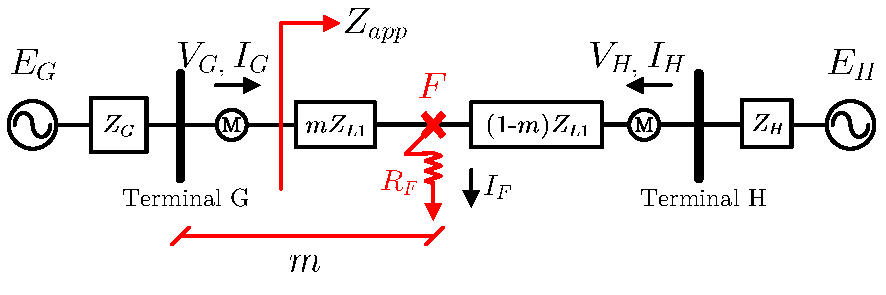
\includegraphics[width=1\columnwidth]{./fig/SistLocFal.pdf}
			\caption{Single line diagram of a transmission system with fault occurring at point F.}
			\label{fig:SistLocFal}
		\end{center}
	\end{figure}
	
	\begin{equation}\label{eq:Zapp}
		\begin{aligned}
			&Z_{app}=\frac{\widehat{V_G}}{\widehat{I_G}}=mZ_{L1}+R_F\left(\frac{\widehat{I_F}}{\widehat{I_G}}\right),
		\end{aligned}
	\end{equation}
	in which $\widehat{V_G}$ and $\widehat{I_G}$ are the fundamental voltage and current phasors recorded at the G terminal of the transmission line in the excited fault loops, given respectively in volts and ampères; $m$ is the distance per unit length in relation to the G terminal; $Z_{L1}$ is the total positive sequence impedance between the terminals of the transmission line, in ohms; $R_F$ is the fault resistance, in ohms; and $I _F$ is the total fault current, in ampères.
	
	Since voltage and current measurements are recorded from a single terminal of the transmission line, (\ref{eq:Zapp}) has three unknowns: $m$, $R_F$ and $\widehat{I_F}$. Fault location methods usually apply simplifications that allow the reduction of unknowns to only one: the distance $m$. The following methods allow the reduction of the effects resulting from $R_F$ and $\widehat{I_F}$ in (\ref{eq:Zapp}) and, therefore, obtaining an estimation of the fault location \cite{Das2014}.
	
	The Reactance method assumes that the fault impedance is purely resistive. Thus, one considers only the imaginary part of the impedances measured, i.e. only the reactance, and the distance $m$ is calculated using:
	
	\begin{equation}\label{eq:mReac}
		\begin{aligned}
			&m=\frac{Im\left(\frac{\widehat{V_G}}{\widehat{I_G}}\right)}{Im(Z_{L1})}.
		\end{aligned}
	\end{equation}
	
	Another technique widely employed is the Takagi method, which introduces a performance gain in relation to the Reactance method. By decomposing the system into a pre-fault circuit and a pure fault circuit, the load current is suppressed from the total fault current and, consequently, the reactance errors from the system load are minimized. In addition, the mathematical formulation obtained reduces the effect of the fault resistance, so that the distance $m$ is computed as:
	
	\begin{equation}\label{eq:mTakagi}
		\begin{aligned}
			&m=\frac{Im(\widehat{V_G}\times\Delta\widehat{I_G}^*)}{Im(Z_{L1}\times\widehat{I_G}\times\Delta\widehat{I_G}^*)},
		\end{aligned}
	\end{equation}
	in which values of $\widehat{V_G}$, $\widehat{I_G}$ and $\Delta\widehat{I_G}$ are chosen accordingly to the excited fault loop, $\Delta\widehat{I_G}$ being the incremental current. For example, assuming a single-phase fault between phase A and ground, one has:
	
	\begin{equation}
		\begin{aligned}
			&\widehat{V_G}=\widehat{V_{AF}},
		\end{aligned}
	\end{equation}
	
	\begin{equation}
		\begin{aligned}
			&\widehat{I_G}=\widehat{I_{AF}}+k\widehat{I_{G0}},
		\end{aligned}
	\end{equation}	
	
	\begin{equation}
		\begin{aligned}
			&\Delta\widehat{I_G}=\widehat{I_{AF}}-\widehat{I_{Apre}},
		\end{aligned}
	\end{equation}
	in which $\widehat{V_{AF}}$ is the phase A fault voltage, recorded at terminal G, in volts; $\widehat{I_{AF}}$ is the fault current in phase A, recorded at terminal G, in ampères; $Z_{L0}$ is the total zero sequence impedance between terminals G and H, in ohms; $\widehat{I_{G0}}$ is the zero sequence current recorded at terminal G, in ampères; and $\widehat{I_{Apre}}$ is the pre-fault current in phase A, recorded at terminal G, in ampères.
	
	Finally, as an evolution of the technique above, alternate versions of the Takagi method, known as Modified Takagi methods, are reported in the literature, which eliminate the need to know the system pre-fault currents. In the zero sequence approach, $\Delta\widehat{I_G}$ is replaced by the zero sequence current $\widehat{I_{G0}}$, and the distance to the fault point is determined by the following equation:
	
	\begin{equation}\label{eq:mTakagiMod}
		\begin{aligned}
			&m=\frac{Im(\widehat{V_G}\times3\widehat{I_{G0}}^*)}{Im(Z_{L1}\times\widehat{I_G}\times3\widehat{I_{G0}}^*)},
		\end{aligned}
	\end{equation}
	
	From equations above, it is expected that any inaccuracies in the transmission line impedances will propagate to short-circuit responses and fault location results. This is investigated in the following section for transmission lines with and without interferences, accounting or not for the soil stratification.
	
	
	\section{CASE STUDY}
	
	A transmission system is proposed in Fig. \ref{fig:Sistema230kV}, composed of a transmission line connecting two equivalent Thévenin circuits. The model was built in the ATP software to perform short-circuit simulations and obtain the current and voltage waveforms, necessary for application of the fault location algorithms. The transmission line operates at 230 kV, with a single circuit, horizontal configuration and, under nominal load conditions, with a current of 500 A per phase. It is assumed a perfect transposition of the conductors. The transmission line is 200 km long and shares the right of way with a 8" diameter underground carbon steel pipeline installed at 1.5 m depth, which runs 10 meters parallel to the transmission line axis along the entire course, as shown in Fig. \ref{fig:SistTesteCorte}. 
	\begin{figure}[hbt]
		\begin{center}
			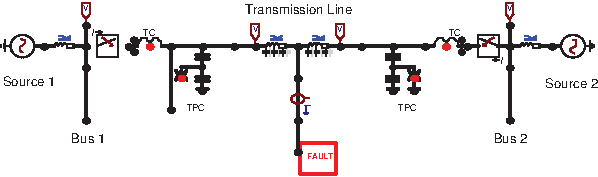
\includegraphics[width=1\columnwidth]{./fig/Sistema230kV2.pdf}
			\caption{ATP model for the short-circuit simulations.}
			\label{fig:Sistema230kV}
		\end{center}
	\end{figure}
	
	\begin{figure}[hbt]
		\begin{center}
			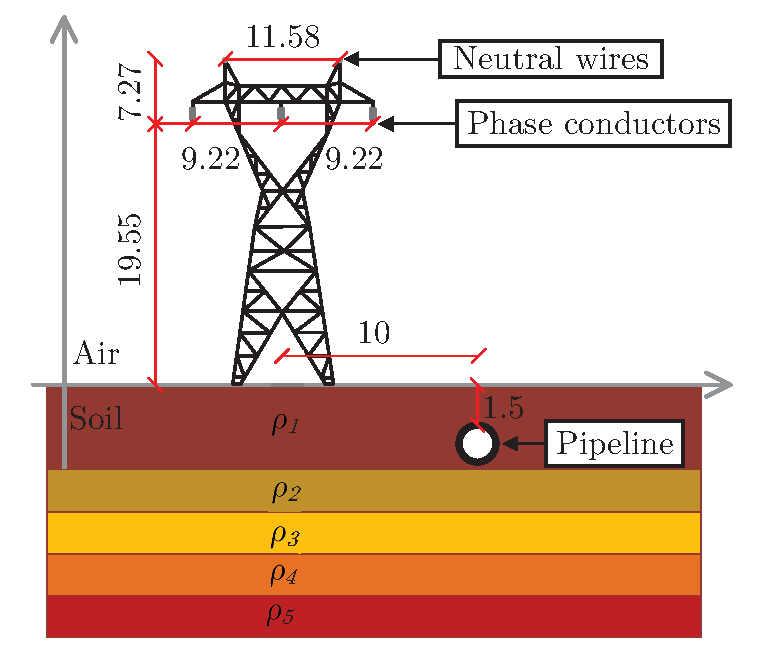
\includegraphics[width=.8\columnwidth]{fig/SistTesteCorte5layers2.pdf}
			\caption{Geometry of the typical tower.}
			\label{fig:SistTesteCorte}
		\end{center}
	\end{figure}
	
	The specifications of the transmission line conductors  are given in Table \ref{table:LTCond}. The pipeline characteristics are provided in Table \ref{table:PipeParam}.
	
	\begin{table}[!hbt]
		\renewcommand{\arraystretch}{1.3}
		\caption{Specifications of transmission line conductors}
		\label{table:LTCond}
		\centering
		\begin{tabular}{|c|c|c|}
			\hline
			\textbf{Conductor} & \textbf{Description} & \textbf{Temperature} \\
			\hline
			Phases & ACSR 636 MCM 27/7 (Peacock) & 50 °C\\
			\hline
			Neutral & Steel 3/8” HS & 50 °C\\
			\hline
		\end{tabular}
	\end{table}
	
	\begin{table}[!hbt]
		\renewcommand{\arraystretch}{1.3}
		\caption{Pipeline characteristics}
		\label{table:PipeParam}
		\centering
		\begin{tabular}{|c|c|}
			\hline
			\textbf{Parameter} & \textbf{Value} \\
			\hline
			Internal radius [m] & 0.1014\\
			\hline
			External radius [m] & 0.1095\\
			\hline
			Electrical resistivity [$\Omega$.m] & $1.72\times10^{-7}$\\
			\hline
			Magnetic permeability [H/m] & $3.77\times10^{-4}$\\
			\hline
		\end{tabular}
	\end{table}
	
	In order to exemplify the effect of the soil resistivity, it is used the apparent resistivity data available in Annex B.3 of the standard ABNT NBR 7117, which describes a soil model stratified in five layers, which parameters are summarized in Fig. \ref{fig:SoilModel} and Table \ref{table:SoilParams} \cite{NBR7117}.
	
	\begin{figure}[hbt]
		\begin{center}
			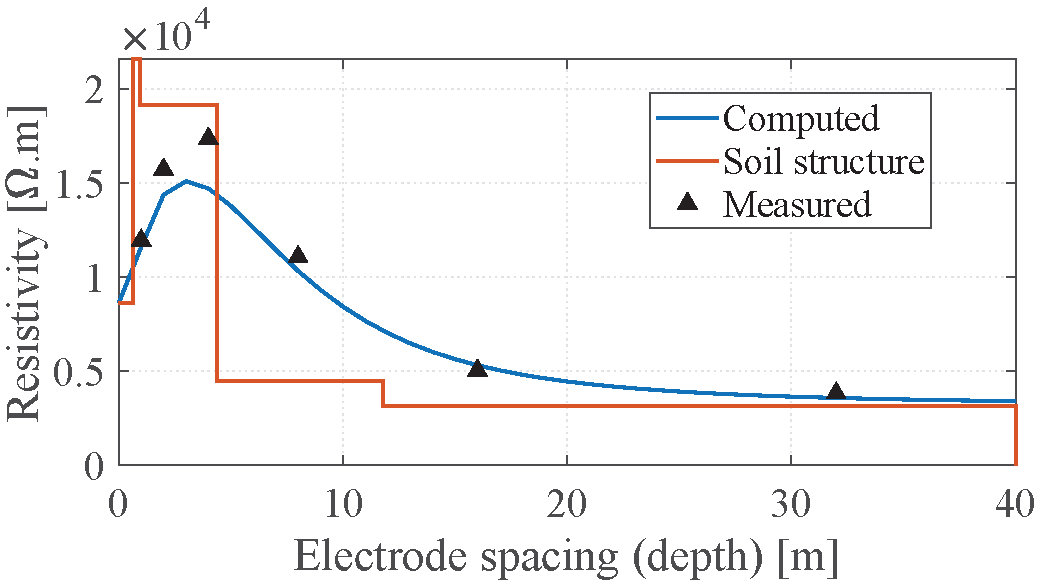
\includegraphics[width=.8\columnwidth]{fig/soilmodel2.pdf}
			\caption{Five-layered soil model as in \cite{NBR7117}.}
			\label{fig:SoilModel}
		\end{center}
	\end{figure}
	
	\begin{table}[]
		\renewcommand{\arraystretch}{1.3}
		\caption{Parameters of the five-layers soil model}
		\label{table:SoilParams}
		\centering
		\begin{tabular}{|c|c|c|c|c|}
			\hline
			\textbf{Layer} & \textbf{\boldmath{$\rho$} {[}\boldmath{$\Omega$}.m{]}} & \textbf{h {[}m{]}} & \textbf{Reflection} & \textbf{Contrast} \\ \hline
			1     & 8600                         & 0.64              & -1.0       & 0.0      \\ \hline
			2     & 21575                        & 0.29              & 0.43       & 2.51     \\ \hline
			3     & 19146                        & 3.47              & -0.06      & 0.89     \\ \hline
			4     & 4460                         & 7.4               & -0.62      & 0.23     \\ \hline
			5     & 3151                         & $\infty$          & -0.17      & 0.71     \\ \hline
		\end{tabular}
	\end{table}
	
	\begin{table}[!hbt]
		\renewcommand{\arraystretch}{1.3}
		\caption{Resistivity values from uniform models}
		\label{table:ResistivityValues}
		\centering
		\begin{tabular}{|c|c|}
			\hline
			\textbf{Model} & \textbf{Resistivity [\boldmath{$\Omega$}.m]} \\
			\hline
			IEEE Std. 80 uniform & 10815\\
			\hline
			RESAP uniform & 9401.48\\
			\hline
			Equivalent uniform & 3160.89\\
			\hline
		\end{tabular}
	\end{table}
	
	Table \ref{table:ResistivityValues} contains three different soil models. In \cite{Martins-Britto2019}, the authors present a formula to represent N-layered soils in terms of a uniform equivalent soil. The standard IEEE Std. 80 defines a uniform soil model as the arithmetic mean of the apparent resistivity values \cite{IEEEStd80}. Finally, the third soil model is obtained through the RESAP module from software CDEGS \cite{Dawalibi1984a}.
	
	Six scenarios are described in order to study the soil models and impacts of EMI:  1) considering IEEE Std. 80 uniform soil and no interferences; 2) considering RESAP uniform soil and no interferences; 3) considering equivalent uniform soil and no interferences; 4) considering IEEE Std. 80 uniform soil and interference caused by a 10 m apart parallel pipeline; 5) considering RESAP uniform soil and interference caused by a 10 m apart parallel pipeline; and 6) considering equivalent uniform soil and interference caused by a 10 m apart parallel pipeline. The case with the equivalent uniform soil model and electromagnetic interferences is considered the most complete case and, for this reason, is the case reference in this paper.
	
	Applying the method described in \cite{Martins-Britto2019} to the parameters of the stratified soil given in Table \ref{table:SoilParams}, a uniform equivalent soil model with resistivity 3160.89 $\Omega$.m is obtained, about 29\% of the result for a uniform model derived directly from the average of the apparent resistivity measurements. It should also be noted that the uniform equivalent resistivity is very close to the value indicated for the deep soil resistivity, which confirms, numerically, reports in the literature that the deep soil resistivity is predominant in studies involving ground return path, and for calculations of mutual couplings in large systems, such as transmission line parameters, the use of the average values of the deep layers often yields satisfactory results for practical purposes \cite{Southey2005}.
	
	Then, the transmission line parameters are calculated and presented in Table \ref{table:LineParam}, for each scenario.
	
	\begin{table}[!hbt]
		\renewcommand{\arraystretch}{1.3}
		\centering
		\caption{Line parameters of the case study for each scenario}
		\begin{tabular}{|c|c|c|}
			\hline
			\textbf{Cases} & \multicolumn{1}{c|}{\textbf{\boldmath{$Z_{1}$ {[}$\Omega$/m{]}}}} & \multicolumn{1}{c|}{\textbf{\boldmath{$Z_{0}$ {[}$\Omega$/m{]}}}} \\ \hline
			1              & 0.1107 + j0.5337                              & 0.5834+j1.8263                                \\ \hline
			2              & 0.1107 + j0.5337                              & 0.5775+j1.8146                                \\ \hline
			3              & 0.1107 + j0.5337                              & 0.5335+j1.722                                 \\ \hline
			4              & 0.1108 + j0.5336                              & 0.3819+j1.3669                                \\ \hline
			5              & 0.1108 + j0.5336                              & 0.38+j1.3628                                  \\ \hline
			6              & 0.1108 + j0.5336                              & 0.3648+j1.329                                 \\ \hline
		\end{tabular}\label{table:LineParam}
	\end{table}
	
	Shunt admittances result in the same values for both calculation methods, with $Y_1$=3.1034j $\mu$S/km and $Y_0$=2.2324j $\mu$S/km, as expected. However, it is observed that there are relevant deviations in zero sequence impedances due to the pipeline presence in the scenarios where the interference is accounted for, presenting a maximum error of 30.81\%. The positive sequence impedance does not show a considerable deviation with respect to interference conditions. The soil model represents less than 3\% of the error in line parameters, showing that, indeed, the presence of interferences tend to more affect impedances than the soil structure. 
	
	In the following sections, short-circuits and fault location algorithms are evaluated, in order to provide a perspective of how these impedance deviations actually influence the power line response and fault locators performance.
	
	\subsection{Short-circuit simulations}
	
	Tables \ref{table:AT_CC} and \ref{table:AT_CC_E} show the short-circuit currents in the fault branch and the corresponding errors for phase-to-ground (AT) simulations occurring at 20\%, 40\%, 60\% and 80\% of the transmission line length, that is, 40 km, 80 km, 120 km and 160 km, using the impedance values obtained for each scenario. The same analysis is performed for phase-to-phase (AB) faults and the respective results are shown in Table \ref{table:AB_CC} and \ref{table:Ab_CC_E}. 
	
	\begin{table}[!hbt]
		\renewcommand{\arraystretch}{1.3}
		\caption{Short-circuit currents for phase-to-ground faults}
		\label{table:AT_CC}
		\centering
		\begin{tabular}{|c|c|c|c|c|}
			\hline
			\textbf{Cases} & \multicolumn{1}{l|}{\textbf{m=20\%}} & \multicolumn{1}{l|}{\textbf{m=40\%}} & \multicolumn{1}{l|}{\textbf{m=60\%}} & \multicolumn{1}{l|}{\textbf{m=80\%}} \\ \hline
			1              & 4190.9 A                              & 3180.1 A                              & 3169.5 A                              & 4149.1 A                              \\ \hline
			2              & 4204.4 A                              & 3191.7 A                              & 3181.1 A                              & 4162.5 A                              \\ \hline
			3              & 4493.8 A                              & 3371.7                                & 3360.5 A                              & 4449 A                                \\ \hline
			4              & 4781.7 A                              & 3698.4 A                              & 3686.1 A                              & 4737 A                                \\ \hline
			5              & 4787.8 A                              & 3703.8 A                              & 3691.5 A                              & 4740 A                                \\ \hline
			6              & 5061.1 A                              & 3859.2 A                              & 3846.3 A                              & 5010.7 A                              \\ \hline
		\end{tabular}
	\end{table}
	
	\begin{table}[!hbt]
		\renewcommand{\arraystretch}{1.3}
		\caption{Short-circuit errors for phase-to-ground faults}
		\label{table:AT_CC_E}
		\centering
		\begin{tabular}{|c|c|c|c|c|}
			\hline
			\textbf{Cases} & \textbf{m=20\%} & \textbf{m=40\%} & \textbf{m=60\%} & \textbf{m=80\%} \\ \hline
			1              & 17.19 \%         & 17.59 \%         & 17.59 \%         & 17.19 \%         \\ \hline
			2              & 16.93 \%         & 17.29 \%         & 17.29 \%         & 16.93 \%         \\ \hline
			3              & 11.21 \%         & 12.63 \%         & 12.63 \%         & 11.21 \%         \\ \hline
			4              & 5.52 \%          & 4.17 \%          & 4.16 \%          & 5.46 \%          \\ \hline
			5              & 5.40 \%          & 4.03 \%          & 4.02 \%          & 5.40 \%          \\ \hline
		\end{tabular}
	\end{table}
	
	\begin{table}[!hbt]
		\renewcommand{\arraystretch}{1.3}
		\caption{Short-circuit currents for phase-to-phase faults}
		\label{table:AB_CC}
		\centering
		\begin{tabular}{|c|c|c|c|c|}
			\hline
			\textbf{Cases} & \textbf{m=20/\%} & \textbf{m=40/\%} & \textbf{m=60/\%} & \textbf{m=80/\%} \\ \hline
			1              & 6539.8 A         & 5015.4 A         & 4998.7 A         & 6474.6 A         \\ \hline
			2              & 6539.6 A         & 5015.4 A         & 4998.7 A         & 6474.6 A         \\ \hline
			3              & 6540 A           & 5015.5 A         & 4998.8 A         & 6474.9 A         \\ \hline
			4              & 6540.5 A         & 5016 A           & 4999.3 A         & 6475.2 A         \\ \hline
			5              & 6540.5 A         & 5016 A           & 4999.3 A         & 6474.9 A         \\ \hline
			6              & 6540.7 A         & 5016.1 A         & 4999.4 A         & 6475.5 A         \\ \hline
		\end{tabular}
	\end{table}
	
	\begin{table}[!hbt]
		\renewcommand{\arraystretch}{1.3}
		\caption{Short-circuit errors for phase-to-phase faults}
		\label{table:Ab_CC_E}
		\centering
		\begin{tabular}{|c|c|c|c|c|}
			\hline
			\textbf{Cases} & \textbf{m=20\%} & \textbf{m=40\%} & \textbf{m=60\%} & \textbf{m=80\%} \\ \hline
			1              & 0.014 \%        & 0.014 \%        & 0.014 \%        & 0.014 \%        \\ \hline
			2              & 0.017 \%        & 0.014 \%        & 0.014 \%        & 0.014 \%        \\ \hline
			3              & 0.011 \%        & 0.012 \%        & 0.012 \%        & 0.009 \%        \\ \hline
			4              & 0.003 \%        & 0.002 \%        & 0.002 \%        & 0.005 \%        \\ \hline
			5              & 0.003 \%        & 0.002 \%        & 0.002 \%        & 0.009 \%        \\ \hline
		\end{tabular}
	\end{table}
	
	Results show that significant discrepancies between the values of short-circuit currents occur only for the phase-to-ground fault, which is expected, since only the zero sequence parameters present differences when considering the interference conditions and the stratified soil. Thus, problems with monitoring devices are expected to arise only in situations in which the fault involves the earth. It should be noted that even for two-phase-to-ground faults, which also involve the earth, monitoring devices do not use zero sequence data, so it can be stated that the impact of pipeline interferences and stratified soil will only exist in events of single-phase faults, which, by the way, are the most common in transmission networks. 
	
	\subsection{Performance of fault locators}
	
	Figure \ref{fig:ConvUniform_NoInterf} and \ref{fig:Conv_StratWithInterf} show the convergence of the fault location algorithms under study, applied to the simulation of a phase-to-ground short-circuit, considering the algorithms set-up in the conventional way, i.e. not including the effects of interferences and soil stratification, for the following scenarios: 1) transmission line with uniform soil and disregarding the interfering pipeline; and 2) transmission line with stratified soil in the presence of interferences.
	
	\begin{figure}[!hbt]
		\begin{center}
			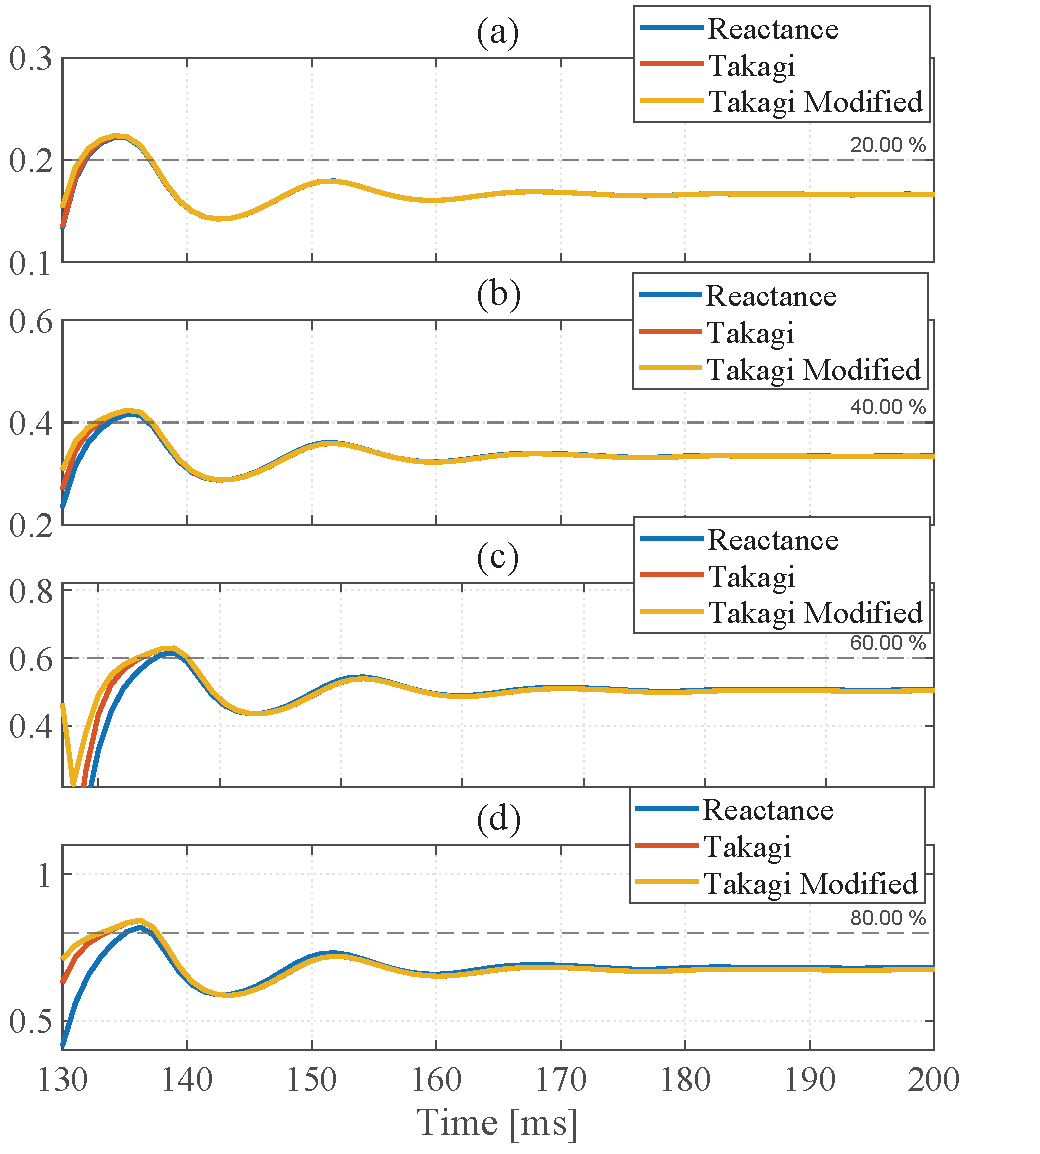
\includegraphics[width=1.1\columnwidth]{./fig/FaultInterfError2.pdf}
			\caption{Estimates of fault location for uniform soil model and disregarding the interfering pipeline, for phase-to-ground fault at: (a) 40 km, (b) 80 km, (c) 120 km and (d) 160 km.}
			\label{fig:ConvUniform_NoInterf}
		\end{center}
	\end{figure}
	
	\begin{figure}[!hbt]
		\begin{center}
			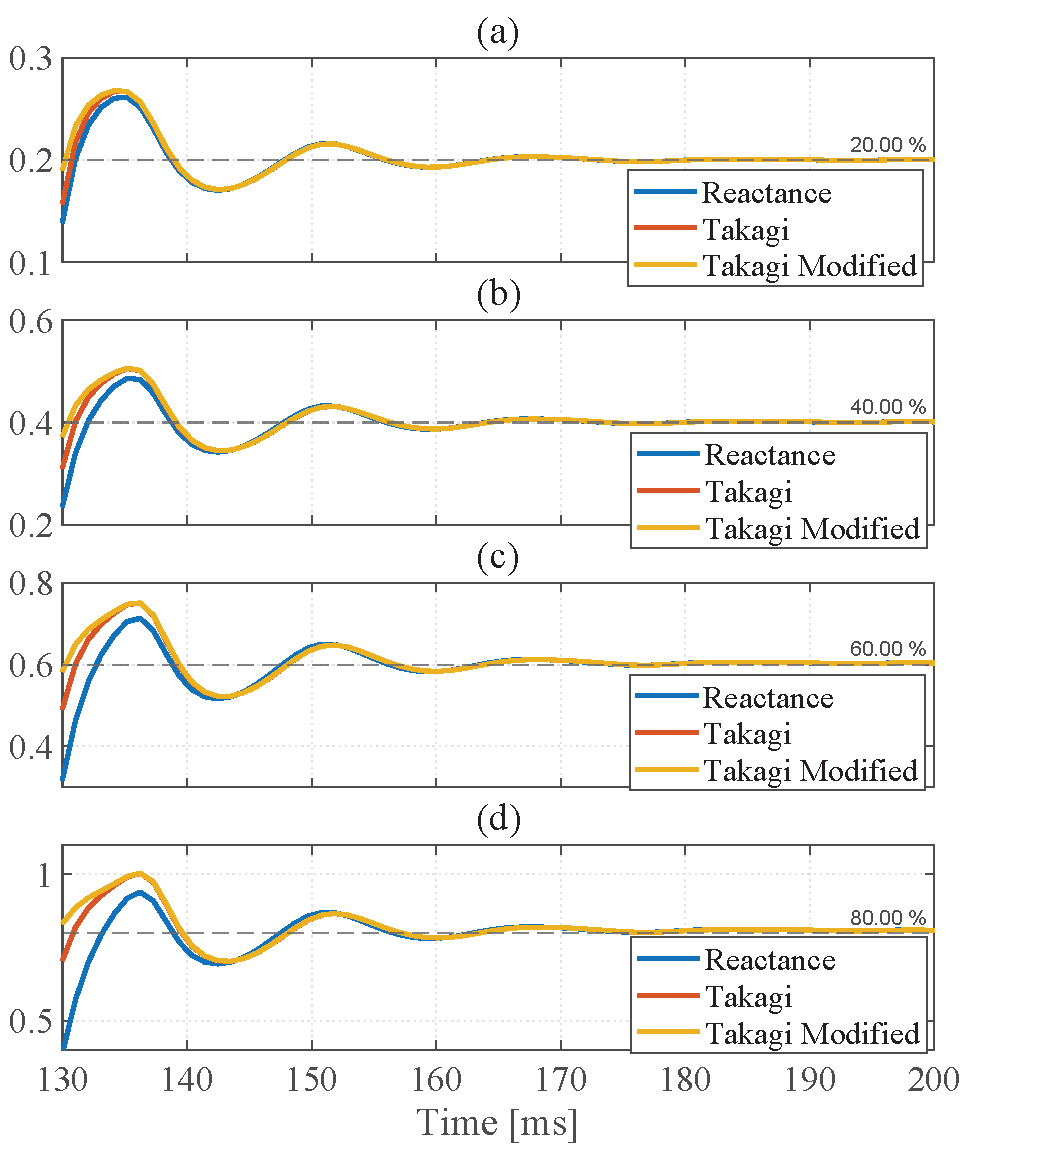
\includegraphics[width=1.1\columnwidth]{./fig/FaultInterf2.pdf}
			\caption{Estimates of fault location for stratified soil model and accounting for the interfering pipeline, for phase-to-ground fault at: (a) 40 km, (b) 80 km, (c) 120 km and (d) 160 km.}
			\label{fig:Conv_StratWithInterf}
		\end{center}
	\end{figure}
	
	Tables \ref{table:Err_UnifNoInt} and \ref{table:Err_StratInt} contain the average location errors for the phase-to-ground fault simulations. In addition, the absolute errors for the evaluated cases of fault location are presented in Fig. \ref{fig:ErrDispersion}, in the form of a scatter plot, in which points located at the lower right and upper left regions represent smaller and larger error situations, respectively, when considering interference conditions.
	
	\begin{table}[!hbt]
		\renewcommand{\arraystretch}{1.3}
		\caption{Fault location errors for phase-to-phase faults, uniform soil, no interferences}
		\label{table:Err_UnifNoInt}
		\centering
		\begin{tabular}{|c|c|c|c|c|}
			\hline
			\textbf{Error} & \textbf{m=20\%} & \textbf{m=40\%} & \textbf{m=60\%} & \textbf{m=80\%}\\
			\hline
			Relative & 0.01\% & 0.1\%  & 0.35\%  & 0.87\%\\
			\hline
			Absolute & 0.02 km & 0.2 km & 0.7 km & 1.74 km\\
			\hline
		\end{tabular}
	\end{table}
	
	\begin{table}[!hbt]
		\renewcommand{\arraystretch}{1.3}
		\caption{Fault location errors for phase-to-phase faults, uniform soil, no interferences}
		\label{table:Err_StratInt}
		\centering
		\begin{tabular}{|c|c|c|c|c|}
			\hline
			\textbf{Error} & \textbf{m=20\%} & \textbf{m=40\%} & \textbf{m=60\%} & \textbf{m=80\%}\\
			\hline
			Relative & 3.36\% & 6.61\%  & 7.95\%  & 12.67\%\\
			\hline
			Absolute & 6.72 km & 13.22 km & 15.9 km & 25.34 km\\
			\hline
		\end{tabular}
	\end{table}
	
	
	\begin{figure}[hbt]
		\begin{center}
			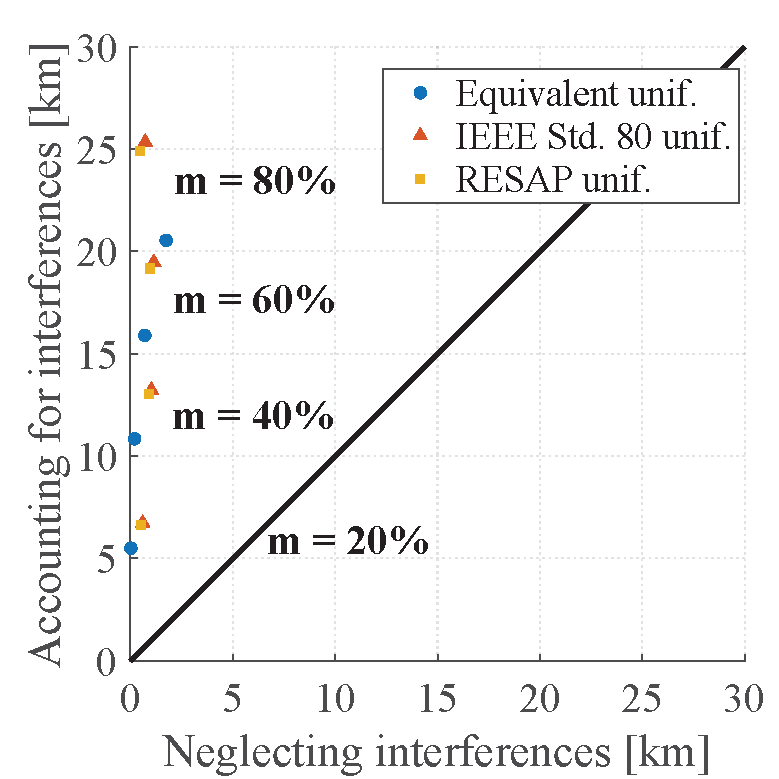
\includegraphics[width=.7\columnwidth]{./fig/dispersao2.pdf}
			\caption{Dispersion of the absolute error for phase-to-ground faults, assuming the presence of the pipeline and stratified soil.}
			\label{fig:ErrDispersion}
		\end{center}
	\end{figure}
	
	Results show that the performance of the fault location algorithms evaluated is impaired when the presence of the pipeline in the vicinity of the transmission line is included, as well as of the stratified soil. In practical situations, as demonstrated, location errors of the order of several kilometers can be verified, causing longer inspection times of the transmission lines to determine the points to be repaired, compromising the system's availability.
	
	\section{CONCLUSIONS}
	
	Results discussed indicate that the discrepancy in the zero sequence impedance propagates to the phase-to-ground short-circuit responses, with an increase of approximately 18\% in the maximum current in the fault branch for the evaluated cases. This value corresponds to about 600 A, an error that is considerably higher than the permissible tolerances for protection devices. There are no significant changes in the cases of phase-to-phase short-circuits.
	
	Likewise, disregarding the soil stratification and interfering structures in the calculation model influences the performance of monitoring algorithms that depend on line parameters, such as fault location methods, especially the one-terminal methods, which depend on the zero sequence line parameters in situations of phase-to-ground faults. From the evaluation of the Modified Takagi and Takagi methods, in the worst case, the location error reaches about 25 km, or 13\% of the length of the transmission line, which may render unviable to apply these localization techniques without considering the effects of interferences with other structures and without building a realistic soil model.
	
	\section*{Acknowledgement}
	This work was developed  in partnership with IATI and CEPEL within the scope of the R\&D project PD-06908-0003/2021, sponsored by the Brazilian Agency of Electrical Energy (ANEEL) and EVOLTZ. The authors thank the cooperation of Ms. Larissa Silva (EVOLTZ) and Dr. Marco Antônio M. Rodrigues (CEPEL).
	
	\bibliographystyle{IEEEtran}
	\nocite{*}
	\bibliography{refs}
	
	
\end{document}
